\documentclass[./thesis.tex]{subfiles}

 
\begin{document}
\label{chap:DET_DRIVEN}

Generally speaking, implementing a wave function method requires iterations over either two-electron integrals, or determinants. Those approaches are referred to as \emph{integral-driven} and \emph{determinant-driven}. Because the number of determinants grows much faster than the number of double excitations, an efficient implementation would likely favor an integral driven approach. However, in most cases, the determinant-driven approach is more intuitive, as it stays closer to the basic CI equations. The \QP is intended for developers, and thus prioritizes the approach that is easier for designing new methods.

For performance, it is vital that some basic operations are done efficiently. Notably, the computation of matrix elements of the Hamiltonian.
This raises some questions about the data structures used to represent the
two-electron integrals and determinants, as well as their consequences from an
algorithmic point of view.

%\begin{itemize}
%\item
%How to store two-electron integrals?
%\item
%How to store determinants?
%\item
%How to compute excitation $\hat T$ so that $\hat T \ket I = \ket J$
%\item
%How to fetch the associated two-electron integral(s)?
%\end{itemize}
%
This chapter is going to address these questions, by going through the basic concepts of our approach to determinant-driven computation.

%\paragraph{Notation}
%\begin{itemize}
%		
%	\item [$\bitI$] : Bitstring representation of $\ket{I}$
%\begin{lstlisting}
%integer*8 :: I(N_int, 2)
%\end{lstlisting}
%	
%	\item [$\bitIsigma$] : 
%	Bitstring representation of $\sigma$ spinorbitals of $\ket{I}$, $\sigma \in \{\uparrow, \downarrow\}$ 
%\begin{lstlisting}
%integer*8 :: Is(N_int)
%\end{lstlisting}
%
%	\item [ {$\bitIsigma [n] $} ] :
%	Bitstring representation of $\sigma$ spinorbitals of $\ket{I}$ in the range $[ 1+n \times 64, \min \qty (n \times 64 + 63, \Norb) ]$, $0 \leq n \leq \Nint-1 \; ;\; \sigma \in \{\uparrow, \downarrow\}$
%\begin{lstlisting}
%integer*8 :: Isn
%\end{lstlisting}
%
%\end{itemize}

%The \QP is built such that the $\uparrow$ and $\downarrow$ spinorbitals share the same space part. In other words, spinorbitals $i$ and $\bar{i}$ both refer to orbital $\phi_i(\br)$.


%----------------------------------------------------------------
\section{Storage of the two-electron integrals}
%----------------------------------------------------------------
\label{sec:integrals}

In all the algorithms presented, all the needed two-electron integrals are kept in memory
and require a fast random access.
A hash table is the natural choice which allows the storage of only non-zero
values with a retrieval of data in nearly constant time,\cite{Maurer1975Mar} but standard hashing
algorithms tend to shuffle the data to limit the probability of collisions.
Here, we favor instead the locality of the data over the probability of collision
using the hash function given in Algorithm~\ref{alg:hash}. It returns the same
value for all the keys which are related by the permutation symmetry of the
indices, keeps some locality in the storage of the data, and can be evaluated
in the order of 10 CPU cycles if the integer division by two is replaced by a
right bit shift instruction.

\begin{algorithm}
 \caption{Hash function that maps the all the quartets of orbital indices related by permutation symmetry to a unique integer.}
 \label{alg:hash}
	\SetKwFunction{FMain}{HASH}
	\SetKwProg{Fn}{Function}{:}{}
\Fn(\tcc*[h]{Hash function for two-electron integrals.}){\FMain{$i,j,k,l$}}{
		\KwData{ $i,j,k,l$ are the orbital indices}
		\KwResult{ The corresponding hash}
        $p \gets \min (i,k)$ \;
        $r \gets \max (i,k)$ \;
        $t \gets p + \frac{1}{2} r (r-1)$ \;
        $q \gets \min (j,l)$ \;
        $s \gets \max (j,l)$ \;
        $u \gets q + \frac{1}{2} s (s-1)$ \;
        $v \gets \min (t,u)$ \;
        $w \gets \max (t,u)$ \;
        \KwRet{$v + \frac{1}{2} w (w-1)$} \;
}
\end{algorithm}

The hash table is such that each bucket can potentially store $2^{15}$
consecutive key-value pairs. The 15 least significant bits of the hash value
are removed to give the index of the bucket ($i_\text{bucket} =
\lfloor \text{hash}(i,j,k,l)/2^{15} \rfloor$), and only those 15 bits need to be
stored in the bucket for the storage of the key ($\text{hash}(i,j,k,l) \mod 2^{16}$).
Hence, the storage of the keys only requires two bytes per key.
The keys within a bucket are sorted in increasing order, enabling a binary
search within the bucket. The search of the key is always fast
since the binary search is bounded by 15 misses and the maximum size of the
array of keys is 64~kiB, the typical size of the L1 cache.

\begin{table}
\caption{Time to access the integrals (in nanoseconds/integral) with different access patterns. The time to generate random numbers (measured as 67~ns/integral) was not counted in the random access results.}
\label{tab:integrals}
\begin{center}
  \begin{tabular}{lrr}
    \hline
   Access  & Array  & Hash table  \\ 
\hline
 $i,j,k,l$ &  9.72  &  125.79     \\ 
 $i,j,l,k$ &  9.72  &  120.64     \\ 
 $i,k,j,l$ & 10.29  &  144.65     \\ 
 $l,k,j,i$ & 88.62  &  125.79     \\ 
 $l,k,i,j$ & 88.62  &  120.64     \\ 
   Random  & 170.00 &  370.00     \\ 
    \hline
  \end{tabular}
\end{center}
\end{table}

% Random function :   6.999999930000001E-008
% Random access :   1.699999983000000E-007
% loop ijkl :   9.719805175081564E-009
% loop ikjl :   1.029155842067460E-008
% loop ijlk :   9.719805175081564E-009
% loop lkji :   8.862175306692014E-008
% loop lkij :   8.862175306692014E-008
%Wall time : 6.72291m

% Random function :   6.999999930000001E-008
% Random access :   3.699999963000001E-007
% loop ijkl :   1.257857140304673E-007
% loop ikjl :   1.446535711350374E-007
% loop ijlk :   1.206399348201300E-007
% loop lkji :   1.257857140304673E-007
% loop lkij :   1.206399348201300E-007
%Wall time : 19.6351m

The efficiency of the storage as a hash table was measured on a dual socket Intel Xeon E5-2680 v2 @ 2.80GHz processor, taking the water molecule with the cc-pVQZ basis set (115 molecular orbitals). The time to access all the integrals was measured by looping over all integrals using different loop orderings. The results are given in table~\ref{tab:integrals}, the reference being the storage as a plain four-dimensional array.

In the array storage,
the value of $170$~ns/integral in the random access case is typical of the latency to fetch a value in the RAM modules when the data is not in any level of cache.
When the data is accessed with a stride of one (the $i,j,l,k$ storage) the cache levels accelerate the access by a factor of $18 \times$, down to $9.71$~ns/integral, corresponding mostly to the overhead of the function call, the retrieval of the data being negligible.

With the hash table, the random access is only $2.18\times$ slower than the random access in the array. Indeed, two random accesses are required: one for the first element of the bucket of keys one for the corresponding value. The rest of the extra time corresponds to the binary search. The locality of the data can be exploited: when the access is done with a regular access pattern, the data is fetched $\sim 3\times$ faster than using a random access.

A CIPSI calculation was run with the array storage and with the hash table storage. With the hash storage, the total wall clock time was increased only by a factor of two.

So to accelerate the access to the most frequently used integrals, all the
integrals involving the $128$ MOs closest to the Fermi
level are copied in a dense array of $128^4$ elements ($2$~GiB).

\section{Internal representation of determinants}
\label{sec:det_representation}

Determinants can be written as a string of creation operators applied to the vacuum state $\vac$.
\begin{equation}
\ac{i} \ac{j} \ac{k} \vac = \ket{I}
\end{equation}
Because of the fermionic nature of electrons, a permutation of two contiguous creation operators results in a sign change, which makes their ordering relevant.
\begin{align}
\ac{j} \ac{i} & = -\ac{i} \ac{j} \\
\ac{j} \ac{i} \ac{k} \vac &=  -\ket{I}
\end{align}
This effectively allows to make any $\Nperm$ permutations
%(even of non-contiguous operators),
and always get $-1^{\Nperm} \ket{I}.$
A determinant can be broken down into two pieces of information:
\begin{itemize}
\item
A set of creation operators, corresponding to the set of occupied spinorbitals in the determinant.
\item
An ordering of the creation operators, responsible for the sign of the determinant. Once an ordering operator $\ordering$ is chosen and applied to all the determinants, it is sufficient to store the sign change that occurs when applying this operator to the string of creation operators. This sign will be referred to as the \emph{phase factor}.
\end{itemize}
Determinants are always associated with a coefficient. So
if the determinants are always built after applying them the same ordering operator,
we don't need to make the phase factor part of the determinant's internal representation. The sign may simply be reported on the associated coefficient.

All the determinants will be built using the order where all the $\uparrow$ spinorbitals are placed before the $\downarrow$ spinorbitals, as in the Waller-Hartree determinant representation:
\begin{equation}
\label{eq:spinpack}
\ordering \ket{I} = \hat{I} \vac = \hat{I}_\uparrow \hat{I}_\downarrow \vac 
\end{equation}
and within each operator $\hat{I}_\uparrow$ and $\hat{I}_\downarrow$, the creation operators are sorted with increasing indices.
For instance, consider the determinant built from the set of spinorbitals $\{i,j,k,{\bar i} \}$ with $i<j<k$,
\begin{equation}
\ket{J} = \ac{j} \ac{k} \ac{\bar i} \ac{i} \vac.
\end{equation}
If we happen to encounter such a determinant, our choice of representation imposes us to consider its re-ordered expression
\begin{equation}
\ordering \ket{J} = - \ac{i} \ac{j} \ac{k} \ac{\bar i} \vac = -\ket{J}
\end{equation}
and the sign change (or \emph{phase factor}) will need to be handled.

The indices of the creation operators (or equivalently the
occupations of the spinorbitals), are stored using the so-called \emph{bitstring} encoding. A bitstring is an array of bits~; typically, the 64-bit binary representation of an integer is a bitstring of size 64.
Quite simply, the idea is to map each spinorbital to a single bit, with a value is set to its occupation number. In other words \texttt{0} and \texttt{1} are associated with the \emph{unoccupied} and \emph{occupied} states.
By this definition, bitstrings encode the indices of the occupied spinorbitals.

For simplicity and performance considerations, the occupations of the $\uparrow$ and $\downarrow$ spinorbitals are stored on different bitstrings, rather than interleaved or otherwise merged in the same one. This allows to straightforwardly map orbital index $n$ to bit index $n-1$ (orbitals are usually indexed from $1$, while bits are indexed from $0$), and makes a bitstring a set of orbitals.
This makes the representation of a determinant a tuple of two bitstrings, associated with respectively $\uparrow$ and $\downarrow$ spinorbitals. Such objects are referred to as \emph{$\uparrow\downarrow$-bitstrings}, and generally define a set of spinorbitals. When used to define a determinant, they imply the previously defined ordering.


\begin{itemize}
\item
$I$ is the $\uparrow\downarrow$-bitstring representation of $\ket{I}$
\item
$I_\uparrow$ is the bitstring representation of the set of occupied $\uparrow$ spinorbitals of $\ket{I}$ 
\item
$I_\downarrow$ is the bitstring representation of the set of occupied $\downarrow$ spinorbitals of $\ket{I}$ 

\end{itemize}


The storage space required for a single determinant is, in principle, one bit per spinorbital, or $2 \times \Norb$ bits. However, because CPUs are designed to handle efficiently 64-bit integers, each spin part is stored as an array of 64-bit integers, the unused space being padded with zeros. 
The actual storage needed for a determinant is $2 \times 64 \times \Nint$ bits, where $\Nint$ is the number of 64-bits integers needed to store one spin part:
\begin{equation}
\Nint = \left \lfloor \frac{\Norb-1}{64} \right \rfloor + 1.
\end{equation}


The Fortran representation of a bitstring is an array of $\Nint$ \lstinline{integer*8} (64-bit integers).  
The Fortran representation of an $\uparrow\downarrow$-bitstring is a two dimensional array of \lstinline{integer*8}, the first dimension of size $\Nint$ and the second of size $2$, corresponding to the $\uparrow$ and $\downarrow$ spin parts.


\lstset{frame=single}
\begin{lstlisting}
  ! I is an updown-bitstring
  ! I_up and I_down are bitstrings
  
  integer*8 :: I(N_int, 2)
  integer*8 :: I_up(N_int), I_down(N_int)

  ... ! load some determinant in I
  I_up   (:) = I(:,1)
  I_down (:) = I(:,2)
\end{lstlisting}
\lstset{frame=none}


In formulas or algorithms, depending on the level of detail desired, a bitstring or $\uparrow\downarrow$-bitstring may also be treated as a single mathematical integer (in $\mathbb{Z}$), avoiding the cumbersome separation into 64-bit packs. However, in algorithms we will usually try to stay closer to the actual implementation. $I$ being the $\uparrow\downarrow$-bitstring associated with $\ket{I}$, we can explicitly refer to a single element of the 64-bit integer array as
\begin{equation}
I_{\sigma}[i]\; ;\; \sigma \in \{\uparrow, \downarrow\}\; ;\; 0 \le i < \Nint
\end{equation}
which is the bitstring representation of the $\sigma$ spinorbitals of determinant $\ket{I}$ in the range $[1+i \times 64, \min \left( (i+1) \times 64, \Norb \right)]$, indexed from $0$ to $63$.

      
\section{Bit manipulation}

The bitstring encoding is a compact way of storing determinants, but it is more than just a data structure. It allows to perform a variety of operations on determinants by taking advantage of CPU's hardware aptitude to perform efficiently bitwise operations on integers.

In many of the presented algorithms, some Fortran intrinsics will be of use. Each of those maps to a CPU instruction that is available on modern CPUs.


\begin{sloppypar}
\begin{itemize}
	      
	\item $\POPCNT{\bitI}$ :
	Returns the number of non-zero bits for a given integer $\bitI$. \\
        ${\POPCNT{\binary{00011000}} = 2}$.
	      
	\item $\TRAILZ{\bitI}$ : Returns the number of trailing zero bits for a given integer $\bitI$. \\
         ${\TRAILZ{\binary{00000100}} = 2}$.
	      
	      
	\item $\IBCLR{\bitI}{n}$ : Returns the value of $\bitI$ with the bit at the $n$-th position set to zero (the rightmost bit is at position zero). \\
        ${\IBCLR{\binary{00001111}}{2} = \binary{00001011}}$.
	      
	     
   	\item $\IOR{\bitI}{\bitJ}$ : Bitwise \texttt{OR} logical operation. \\
        ${\IOR{\binary{1100}}{\binary{1010}} = \binary{1110}}$.

	 
	\item $\IEOR{\bitI}{\bitJ}$ : Bitwise \texttt{XOR} (exclusive or) logical operation. \\
        ${\IEOR{\binary{1100}}{\binary{1010}} = \binary{0110}}$.
	      
	      
	\item $\IAND{\bitI}{\bitJ}$ : Bitwise \texttt{AND} logical operation. \\
        ${\IAND{\binary{1100}}{\binary{1010}} = \binary{1000}}$.
	      
	      
	\item $\NOT{\bitI}$ : Bitwise \texttt{NOT} logical operation. \\
        ${\NOT{\binary{00001100}} = \binary{11110011}}$.
	      
	\item $\ISHFT{\bitI}{n}$ : Returns $\bitI$ with bits shifted $|n|$ places to the left if $n>0$, otherwise to the right. Bits shifted out of the range are lost. Zeros are shifted from the opposite end. \\
        ${\ISHFT{\binary{01001110}}{2} = \binary{00111000}}$, \\
        ${\ISHFT{\binary{01001110}}{-2} = \binary{00010011}}$.
	      
	\item $\BTEST{\bitI}{n}$ : Returns $\TRUE$ if the $n$-th bit of $\bitI$ is set, otherwise $\FALSE$. \\
        $\BTEST{\binary{00001000}}{3} = \TRUE$.
	      
\end{itemize}
\end{sloppypar}
      
      
Those intrinsics apply to integers with at most 64-bits. This however is a purely implementational limitation, so depending on the level of detail desired, this constraint can be unambiguously lifted in formulas or algorithms. Different notations will be used for the 64-bit and the $\mathbb{Z}$ cases, as they are not always equivalent.
For example, the $\ISHFT{\_}{\_}$ Fortran intrinsic always returns zero for shifts larger than 64 bits, which is not the case for the $\ishft{\_}{\_}$ function over mathematical integers.
%So it is convenient to introduce functions and notations acting on mathematical integers.
All binary operators are of same precedence and left-associative.

\begin{center}
  \begin{tabular}{l@{\hskip 10ex}l}
\hline
  64-bit variant  &  mathematical variant \\
\hline
    $\ISHFT{\bitI}{n}$ & $\ishft{I}{n}$  \\ 
    $\TRAILZ{\bitI}$ & $\trailz{I}$  \\ 
    $\IBCLR{\bitI}{n}$ & $\ibclr{I}{n}$  \\ 
    $\BTEST{\bitI}{n}$ & $\btest{I}{n}$  \\ 
    $\NOT{\bitI}$ & $\neg I $  \\ 
    $\IAND{\bitI}{\bitJ}$ & $\iand{I}{J}$ \\
    $\IOR{\bitI}{\bitJ}$ & $\ior{I}{J}$ \\
    $\IEOR{\bitI}{\bitJ}$ & $\ieor{I}{J}$ \\
    $\POPCNT{\bitI}$ & $\popcnt{I}$ \\
\hline
  \end{tabular}
\end{center}


Some examples of how these instructions can be used are given below. They are key to understand how we can determine the holes and particles involved in the $\excdet{I}{J}$ excitation operator defined by
\begin{equation}
\label{eq:ordering_removed}
\ket{J} = \excdet{I}{J} \ket{I}.
\end{equation}
Let $\bitI$ and $\bitJ$ be the bitstring representations of $\ket{I}$ and $\ket{J}$, and $\bit{P}$ a bitstring with $\Nint=1$. 


\begin{itemize}
	      
	\item $I_{\uparrow}$ : bitstring representation of the set of $\uparrow$ spinorbitals of $\ket{I}$
	            
	\item $\popcnt{I_{\uparrow}}$ : number of spinorbitals in $I_{\uparrow}$ (equal to the number of $\uparrow$ electrons).
	            
	\item $\ieor{I_{\uparrow}}{J_{\uparrow}}$ : bitstring representation of the set of $\uparrow$ spinorbitals that are present in either $I_{\uparrow}$ or $J_{\uparrow}$, but not in both (exclusive disjunction).
        This operator identifies all the $\uparrow$ spinorbitals involved in the excitation from $\ket{I}$ to $\ket{J}$. 
	            
	\item $\iand{I_{\uparrow}}{\qty(\ieor{I_{\uparrow}}{J_{\uparrow}})}$ : 
        bitstring representation of the set of $\uparrow$ spinorbitals of $\ket{I}$ involved in the excitation from $\ket{I}$ to $\ket{J}$. This corresponds to the indices of the holes in the excitation $\excdet{I}{J}$ or to the particles in $\excdet{J}{I}$. 
	            
	\item $\popcnt{\ieor{I_{\uparrow}}{J_{\uparrow}}}/2$ : because the excitation of an electron involves 2 spinorbitals (one hole and one particle), this is the $\uparrow$ excitation degree between $\ket{I}$ and $\ket{J}$.
	            
	\item $\TRAILZ{\bit{P}}+1$ : the index of the lowest orbital in $\bit{P}$ if $\bit{P} \ne 0$. If $\bit{P} = 0$, this function returns $65$.
	            
	\item $\IBCLR{\bit{P}}{\TRAILZ{\bit{P}}}$ : $\bit{P}$ without its orbital of lowest index.

\end{itemize}


\section{Identification of holes and particles}
\label{sec:det_exc}

An algorithm used to compute the excitation degree is presented as algorithm \ref{alg:EXC_DEGREE}, and one to compute the sets of created holes and particles as algorithm \ref{alg:EXC}. Algorithm \ref{alg:EXC}, however, returns the sets as bitstrings. Extracting the indices from a bitstring is another basic operation, presented as algorithm \ref{alg:LIST_FROM_BITSTRING}.
Because computing excitations is a hotspot of the program, and because we are typically interested in double excitations at most, a more specialized algorithm can be used.\cite{Scemama_2013}


\begin{algorithm}[h!]
	\caption{Returns the degree of excitation between two determinants.}
	\label{alg:EXC_DEGREE}
	\SetKwFunction{FMain}{EXC\_DEGREE}
	\SetKwProg{Fn}{Function}{:}{}
	
	\Fn(){\FMain{$I, J$}}{
		\KwData {$I, J$: bitstring representations of determinants $\ket{I}$ and $\ket{J}$. }
		\KwResult{ Returns the excitation degree between $\ket{I}$ and $\ket{J}$, namely $\frac{1}{2}\popcnt{\ieor{I}{J}}$ }

		$X \gets 0$   \;
		\For{$\sigma \in \{\uparrow, \downarrow\}$}{
		\For{$i \gets 0,  \Nint-1$}{
		  $X \gets X+\POPCNT{\IEOR{I_{\sigma}[i]}{J_{\sigma}[i]}}$  \;
		}
		}
		\KwRet $X / 2$\;
	}
\end{algorithm}


\begin{algorithm}[H]
	\caption{Returns the holes and particles created in an excitation as bitstrings.}
		
	\SetKwFunction{FMain}{EXC}
	\label{alg:EXC}
	\SetKwProg{Fn}{Function}{:}{}
	
	\Fn(){\FMain{$I$,$J$}}{
	\KwData{ $I, J$: the bitstring representations of determinants $\ket{I}$ and $\ket{J} = \excdet{I}{J} \ket{I}$}
	\KwResult{ Returns a tuple $(P,H)$, where $P$ and $H$ are respectively the sets of particles and holes created by $\excdet{I}{J}$, as $\uparrow \downarrow$-bitstrings.  }
		\For{$\sigma \in \{\uparrow, \downarrow\}$}{
		\For{$i \gets 0, \Nint-1$}{
			$C \gets \IEOR{I_{\sigma}[i], J_{\sigma}[i]}$\;
			$P_{\sigma}[i] \gets \IAND{C, J_{\sigma}[i]}$\;
			$H_{\sigma}[i] \gets \IAND{C, I_{\sigma}[i]}$\;
		}
		}
		\KwRet{ $(P,H)$}\;
		}
\end{algorithm}




\begin{algorithm}[h!]
	\caption{Transforms a bitstring into a list of orbital indices.}
	\label{alg:LIST_FROM_BITSTRING}
	\SetKwFunction{FMain}{LIST\_FROM\_BITSTRING}
	\SetKwProg{Fn}{Function}{:}{}
	
	\Fn(){\FMain{$P$}}{
		\KwData{ $P$ a bitstring. On output, $P$ is destroyed. }
		\KwResult{ $L$ the list of orbital indices in $P$ in increasing order.}
		$k \gets 0$ \;
		\For{$i \gets 0, \Nint-1$}{
		\While{$P[i] \neq 0$}{
		$e \gets \TRAILZ{P[i]}$ + 1\;
		$P[i] \gets \IBCLR{P[i]}{e}$\;
		$L[k] \gets e + i \times 64$\;
                $k \gets k+1$\;
		}
                \tcc{$L$ contains $k$ elements}
		\KwRet{$L$}
		}
		}
		
\end{algorithm}



\section{Phase factors}


The computation of phase factors is slightly more complex. The following explanation is limited to one spin part. More detail will be given later about why spin parts can be treated independently.
As we have seen in section~\ref{sec:det_representation}, the $\uparrow \downarrow$-bitstring representation of determinants implies an ordering of creation operators : first all the $\uparrow$ operators, then all the $\downarrow$, both with increasing orbital indices.

Whenever we build a new determinant by applying an excitation operator, we obtain a determinant that is initially expressed not just with a different ordering, but with a mix of creation and annihilation operators.

First of all, we have to make this initial expression unambiguous by precisely defining excitation operators. We have defined an implicit ordering for the expression of determinants, we also need an implicit ordering for the expression of excitation operators.
Like for determinants, we pack together $\uparrow$ and $\downarrow$ operators.
\begin{equation}
\label{eq:spinpackexc}
\hat T = \hat T_\uparrow \hat T_\downarrow.
\end{equation}
Within $\hat T_\uparrow$ and $\hat T_\downarrow$, the creation and annihilation operators are separately sorted with increasing indices, then interleaved starting with a creation. In other words, $\hat T_\uparrow$ and $\hat T_\downarrow$ are written as a products of single excitations, lowest particle with lowest hole, then second lowest particle with second lowest hole, \textit{etc}, and we arbitrarily chose to put creation before annihilation operators.
For example, the double excitation $\excorb{ab}{cd}$ with $a<b<c<d$ is expressed as
\begin{equation}
\hat T_{ab}^{cd} = \ac{c} \an{a} \ac{d} \an{b} = \hat T_a^c \hat T_b^d.
\end{equation}

We can now express $\hat T$ as a series of operators.
In most cases, permuting contiguous operators will still just result in a sign change.
\begin{align}
\an{j} \an{i} & = -\an{i} \an{j} \\
\ac{j} \an{i} & =
  \begin{cases}
  -\an{i} \ac{j} & i \ne j \\
  1 - \an{i} \ac{i} & i = j.
  \end{cases}
\end{align}
A particular case is the permutation of a creation and an annihilation operator with the same index.
Indeed, if spinorbital $l$ is unoccupied in $\ket{I}$,
\begin{align}
\label{eq:aa+}
\an{l} \ac{l} \ket{I} & = \ket{I}  \\
\ac{l} \an{l} \ket{I} & = 0 .
\end{align}
In the first case, a particle is created then annihilated, resulting in the same determinant. In the second case, there is an attempt at annihilating a particle that does not exist, resulting in $0$. It is of course the opposite if $l$ is occupied in $\ket{I}$.
These formulas will be used to remove annihilation operators from the expression of a determinant.


Let $\ket{I}$ and $\ket{K}$ be two determinants with spinorbitals ordered as in the $\uparrow \downarrow$-bitstring  representation:
\begin{align}
\ket{I} & = \ac{i}\ac{j}\ac{k} \vac \\
\ket{K} & = \ac{i}\ac{k}\ac{l} \vac
\end{align}
with $i<j<k<l$.
When one applies the excitation operator $\excorb{j}{l}$ to $\ket{I}$,
\begin{equation}
\excorb{j}{l} \ket{I} = \ac{l} \an{j} \ac{i} \ac{j} \ac{k} \vac.
\end{equation}
To build the corresponding $\uparrow \downarrow$-bitstring, one needs to
reorder the operators by permuting contiguous operators.
It takes $n=1$ permutation to bring $\an{j}$ behind $\ac{j}$:
\begin{equation}
\excorb{j}{l} \ket{I} = -\ac{l} \ac{i} \an{j} \ac{j} \ac{k} \vac.
\end{equation}
Using equation~\ref{eq:aa+},
\begin{equation}
\excorb{j}{l} \ket{I} = -\ac{l} \ac{i} \ac{k} \vac.
\end{equation}
Then, it takes again $n$ permutations to bring $\ac{l}$ to the position formerly occupied by $\ac{j}$, and $x=1$ more permutation to bring it at its final position.
\begin{equation}
\excorb{j}{l} \ket{I} = -\ac{i} \ac{k} \ac{l} \vac = -\ket{J}.
\end{equation}

The total number of permutations needed is $\Nperm = 2n+x$. The parity of $\Nperm$ is the parity of $x$. As can be seen, $x$ is the number of spinorbitals with indices in the $]j, l[$ range in $\ket{I}$ (regardless of whether $l>j$ or $l<j$). In our case, there was one occupied spinorbital $k$, so $\Nperm$ is odd and we ended with a negative phase factor, $-1^\Nperm=-1$.

\begin{figure}[h!]
	\begin{center}
		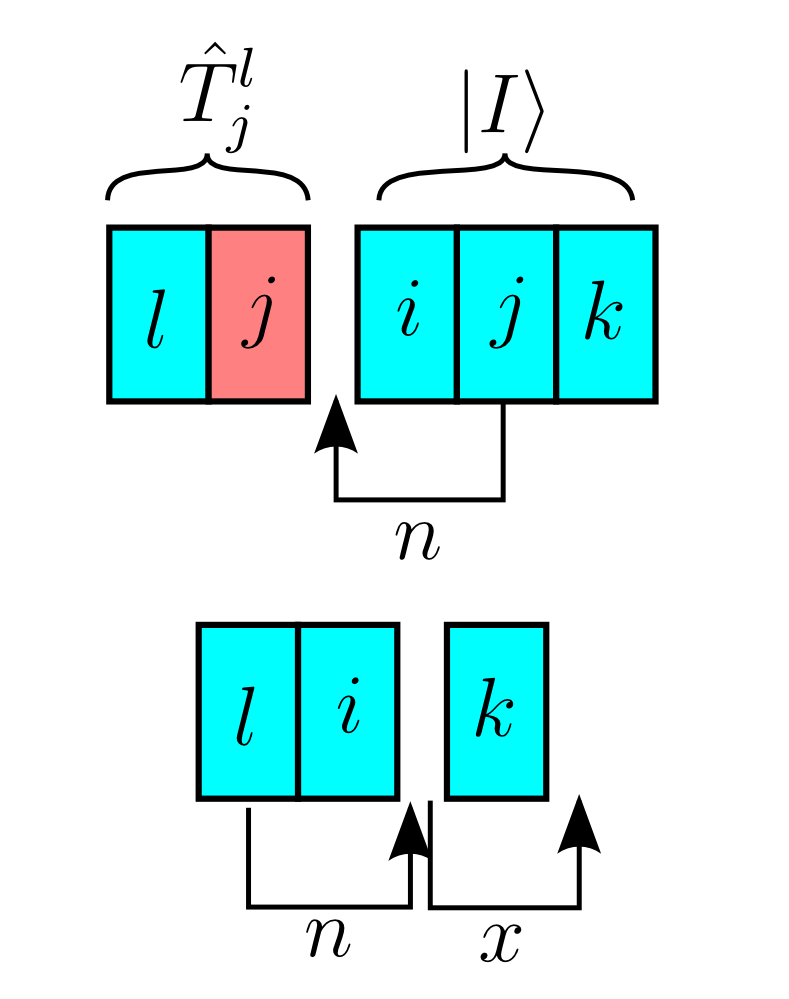
\includegraphics[width=0.25\columnwidth]{figures/determinant_driven/phasefactor}
	\end{center}
	\caption{ \label{fig:phasefactor} Computation of the phase factor.}
\end{figure}

\subsection{Treating spin parts separately}

It is not immediately obvious that $\uparrow$ and $\downarrow$ spin parts can be treated independently. It is possible because our ordering packs together operators of same spin in the expression of both determinants (Eq.~\eqref{eq:spinpack}) and excitations (Eq.~\eqref{eq:spinpackexc}), and 
also because we never consider excitations where the spin is changed (spin-flips).
% redondant avec l'eq 11
%Under these constraints, any excitation operator $\hat{T}$ can be expressed as 
%\begin{equation}
%\hat{T} = \hat{T}_\uparrow \hat{T}_\downarrow .
%\end{equation}

\begin{align}
\label{eq:spin1}
\hat{T} \ket{I} & = \hat{T}_\uparrow \hat{T}_\downarrow \,  \hat{I}_\uparrow \hat{I}_\downarrow \vac \\
\label{eq:spin2}
            & =  \qty(\hat{T}_\uparrow \hat{I}_\uparrow) \qty(\hat{T}_\downarrow  \hat{I}_\downarrow) \vac 
              = \hat{J}_\uparrow \hat{J}_\downarrow  \vac = \pm \ket{J}.
\end{align}

The number of creation and annihilation operators in an excitation operator is always even. Hence, going from Eq.~\eqref{eq:spin1} to Eq.~\eqref{eq:spin2} by permuting $\hat{T}_\downarrow$ with $\hat{I}_\uparrow$ always requires an even number of permutations, keeping the phase factor unchanged.
So the phase factors can be easily computed by reordering separately $\hat{T}_\uparrow \hat{I}_\uparrow$ and $\hat{T}_\downarrow  \hat{I}_\downarrow$.



\subsection{Single excitations}

%In the case of a single excitation, only one spin part is involved. All indices refer to spinorbitals of same, arbitrary spin $\sigma \in \{\uparrow, \downarrow\}$

For a given determinant $\ket{I}$ and a singly excited determinant $\ket{J} = \ordering \excorb{i'}{j'} \ket{I}$ where both 
use the ordering of spinorbitals defined previously, the phase factor can be determined by the parity of
\begin{equation}
N^{I}_{ij}=\sum_{k=i+1}^{j-1} \occ{k}{I}
\end{equation}
where $i=\min(i',j')$, $j=\max(i',j')$ and
\begin{equation}
\occ{k}{I} = \delta \qty(\ac{k}\an{k} \ket{I} - \ket{I}) = \begin{cases}
 1 & \text{if } \ac{k}\an{k} \ket{I} = \ket{I} \\
 0 & \text{otherwise}
\end{cases}
\end{equation}
is the occupation number of spinorbital $k$ in determinant $\ket{I}$.\footnote{Note that occupation
numbers in $\ket{I}$ and $\ket{J}$ are by construction equal for any spinorbital $k \neq i \neq j$, so while we will use $\ket{I}$ in the following, we could as well use $\ket{J}$.
%This is obvious from the fact that $\Hij{I}{J}=\Hij{J}{I}$.
}
We will use the fact that the parity of an integer $X$ can be obtained by extracting the least significant bit of its binary representation: 
\begin{equation}
p(X)=\iand{X}{1} = \begin{cases}
1 & \text{ if $X$ is odd  } \\
0 & \text{ if $X$ is even.} 
\end{cases}.
\end{equation}


A bitstring $R_{ij}$, containing all orbitals in a given range $]i, j>i[$ can be built as 
\begin{equation}
R_{ij}=\ieor{\ishft{\neg{0}}{i}}{\ishft{\neg{0}}{j-1}}
\end{equation}
where $\neg{0}$ denotes the bitstring where all the bits are set to one.

Let $I$ be the bitstring representation of $\ket{I}$, the number of $\sigma$-spinorbitals in $\ket{I}$ in the given orbital range can be evaluated as
\begin{equation}
N^{I}_{ij} = \popcnt{\iand{I_{\sigma}}{R_{ij}}}.
\end{equation}
So the phase factor to be applied when going from $\ket{I}$ to $\ket{J}$ is 
\begin{equation}
\phase{\ket{I}}{\ket{J}} = -1^{p(N^I_{ij})}.
\end{equation}
Using the above formulas and taking into account the internal representation of $\uparrow \downarrow$-bitstring as arrays of $\Nint$ \lstinline{integer*8}, we get algorithm~\ref{alg:PHASE_SINGLE}.   


\begin{algorithm}
	\caption{Returns the phase factor of $\ordering \excorb{a}{b} \ket{I}$.}
	\label{alg:PHASE_SINGLE}
				\SetKwFunction{FMain}{PHASE\_SINGLE}
	\SetKwProg{Fn}{Function}{:}{}
	
	\Fn(){\FMain{$I_\sigma, a, b$}}{
		\KwData{ $I_\sigma$ the bitstring representation of $\sigma \in \{\uparrow, \downarrow\}$ spinorbitals of $\ket I$}
		\KwData{ $a,b$ indices of a hole and a particle created in $\sigma$ spinorbitals of $\ket I$ }
		\KwResult{ The phase factor associated with $\ordering \excorb{a}{b} \ket{I}$}
		$\texttt{high} \gets \max(a,b)-1$ \;
		$\texttt{low} \gets \min(a,b)-1$ \;
		$il \gets \frac{\texttt{low}}{64}$ \;
		$ih \gets \frac{\texttt{high}}{64}$ \;
		$l \gets \texttt{low} \mod 64$ \;
		$h \gets \texttt{high} \mod 64$ \; 
		\For{$i \gets il, ih-1$}{
			$\texttt{mask}[i] = \texttt{NOT}(0)$\;		
		}

		%$mask[ih] \gets ISHFT(NOT(0), h-63)$ \;
		%$mask[il] \gets IAND(mask[il], ISHFT(NOT(0), l))$ \;
		
		$\texttt{mask}[ih] \gets \texttt{ISHFT}(\texttt{NOT}(0), h+1)$ \;
		$\texttt{mask}[il] \gets \texttt{IEOR}(\texttt{mask}[il], \texttt{ISHFT}(\texttt{NOT}(0), l))$ \;
		
		
		$\Nperm \gets 0$ \;
		\For{$i \gets il,ih$}{
			$\Nperm \gets \Nperm + \texttt{POPCNT}(\texttt{IAND}(I_{i}, \texttt{mask}[i]))$ \;
		}
                $\texttt{phase}[0:1] = [ 1.0 \;;\; -1.0 ]$ \;
                \KwRet $\texttt{phase}[\texttt{IAND}(\Nperm,1)]$ \;
		}
\end{algorithm}


\subsection{Phase masks}
\label{chap:PHASEMASK}

Algorithm \ref{alg:PHASE_SINGLE} is a general one, efficient for computing the phase factor for arbitrary determinants. However, a phase computation is typically needed every time two determinants are compared, resulting in a vast amount of computational power being consumed. When only this method was used in the \QP, it was not uncommon to find that a large fraction of the computational time was spent in phase computations.
Advantage can be taken of the fact that, in most cases, the considered determinants aren't actually arbitrary. Usually, the phase computation will be performed repeatedly with the same determinant. For a fairly modest computational price, it is possible to compress the phase information from a particular determinant and make it cheaper to extract. The underlying principle is little more than a cumulative sum. If, for a determinant $\ket{I}$ that is going to be used repeatedly for phase computations, we pre-compute
\begin{equation}
E^I_i = \sum_{k=1}^{i} \occ{k}{I}
\end{equation}
we can access $N^I_{ij}$ for any $i$ and $j>i$ with no need to loop over $k$ as
\begin{equation}
N^I_{ij} = E^I_{j-1} - E^I_{i}.
\end{equation}


This requires to store $E^I$ which is an integer array of size $2 \times (\Norb+1)$. This may be somewhat memory consuming if we want to pre-compute and store $E$ for each determinant. However, because the actual information needed isn't $N^I_{ij}$, but merely its parity, we only need to store the so-called ``phase mask'' array $P^I$
\begin{equation}
\label{eq:phasemask}
P^I_i = p(E^I_i)
\end{equation}
which is 1 bit of information per spinorbital, as opposed to an integer big enough to accommodate a number of electrons.
\begin{align}
E^I_i & = 2 \times  \Big \lfloor \frac{E^I_i}{2} \Big \rfloor + P^I_i \\
N^I_{ij} & = E^I_{j-1} - E^I_{i} \\
 & = 2 \times \qty( \Big \lfloor \frac{E^I_{j-1}}{2} \Big \rfloor - \Big \lfloor \frac{E^I_{i}}{2} \Big \rfloor ) + P^I_{j-1} - P^I_{i}
\end{align}
	    
In the last equation, $N^I_{ij}$ is expressed as a sum of three terms. The first one being even by construction, the parity of $N^I_{ij}$ is the parity of the rest of the sum:
\begin{equation}
p(N^I_{ij})=p(P^I_{j-1} - P^I_{i})
\end{equation}
This can be rewritten in a slightly more efficient way as
\begin{equation}
p(N^I_{ij}) = P^I_{j-1} \oplus P^I_{i}
\end{equation}

%Note that using $E^I$ instead of $P^I$ would require an extra ADD instruction ( totalement negligeable ? )
%\begin{equation}
%p(N^I_{ij}) = (E^I_{i+1} - E^I_j) \wedge 1
%\end{equation}

We have used sorted indices $i<j$. In practice, we know which index refers to the particle and which refers to the hole. With an excitation operator $\hat T_h^p$ applied to $\ket {I}$, noticing that

\begin{itemize}
\item
if $p>h$ we have
\begin{align}
p(N^I_{hp}) &= P^I_{p-1} \oplus P^I_{h} \\
& = P^I_{p} \oplus P^I_{h} \oplus \occ{p}{I} \\
& = P^I_{p} \oplus P^I_{h} 
\end{align}

\item
if $h>p$ we have
\begin{align}
p(N^I_{ph}) &= P^I_{h-1} \oplus P^I_{p} \\
& = P^I_{h} \oplus P^I_{p} \oplus \occ{h}{I} \\
& = P^I_{h} \oplus P^I_{p} \oplus 1
\end{align}

\end{itemize}

the phase factor can be computed as
\begin{align}
\label{eq:PHASE_FACTOR}
\phase{\ket{I}}{\ordering \hat T_h^p \ket{I}} = 
\begin{cases}
(-1)^{P^I_{h} \oplus P^I_{p}} & \text{if } p>h \\
-(-1)^{P^I_{h} \oplus P^I_{p}} & \text{if } h>p \\
\end{cases}
\end{align}


\begin{algorithm}
	\caption{Returns a phase mask as a bitstring.}
	\label{alg:PHASEMASK}	
	\SetKwFunction{FMain}{PHASEMASK}
	\SetKwProg{Fn}{Function}{:}{}
	
	\Fn(){\FMain{$\bitI$}}{
		\KwData{ $\bitI$ the bitstring representation of $\ket{I}$}
		\KwResult{ $\bitP$ is the phase mask associated with $\ket{I}$, as described in Eq.~\eqref{eq:phasemask}, as a bitstring.}
		   
		\For{$\sigma \in \{\uparrow, \downarrow\}$}{
		$r \gets 0$ \;
		\For{$i \gets 0, N_{int}-1$}{
				$\bitPsigma[i] \gets \texttt{IEOR}(\bitIsigma[i], \text{ISHFT}(\bitIsigma[i], 1)$ \;
				\For{$d \gets 0, 5$}{
					$\bitPsigma[i] \gets \text{IEOR}(\bitPsigma[i], \text{ISHFT}(P_\sigma[i], 2^d)$ \;
				}
				$\bitPsigma[i] \gets \texttt{IEOR}(\bitPsigma[i], r)$ \;
				\If{$\texttt{IAND}(\texttt{POPCNT}(\bitIsigma[i]), 1) == 1$}{
					$r \gets \texttt{NOT}(r)$ \;			
				}
			}
		}
		%\tcc{Ignoring the shift will cause all phases to be flipped, which is transparent.}
		%$P = \ishft{P}{1}$ \;
		\KwRet{$P$} \;
		}
\end{algorithm}



\begin{algorithm}
	\caption{Returns a phase factor associated with a single excitation using a phase mask. This routine may be optimized by replacing the integer divisions by bit shifts and the modulo by an \texttt{AND} instruction.}
	\label{alg:PHASE_FROM_PHASEMASK}	
	\SetKwFunction{FMain}{PHASE\_PHASEMASK}
	\SetKwProg{Fn}{Function}{:}{}
	
	\Fn(){\FMain{$P^I$, $i$, $j$}}{
		\KwData{ $P^I$ is the phase mask array associated with $\ket{I}$, as described in Eq.~\eqref{eq:phasemask}. $i$ and $j$ are spinorbitals of spin $\sigma \in \{\uparrow, \downarrow \}$ so that $\excorb{i}{j} \ket{I} \neq 0 $.}
		\KwResult{ The phase factor associated with $\ordering \excorb{i}{j} \ket{I}$.}

		\uIf{$j < i$}{
			$c \gets 0$ \;
		}
		\Else{
			$c \gets 1$ \;		
		}
		$i_n \gets (i-1)/64$ \;
		$j_n \gets (j-1)/64$ \;
		$i_b \gets (i-1) \mod 64$ \;
		$j_b \gets (j-1) \mod 64$ \;
		$B \gets \ISHFT{P_\sigma^I[i_n]}{-i_b} \oplus \ISHFT{P_\sigma^I[j_n]}{-j_b}$ \;
		\uIf{$B \wedge 1 = c$}{
		\KwRet{ $-1$}\;}
                \Else{\KwRet{ $1$} \; }
        
        
		%\uIf{$\qty(P^I_\sigma[i+1] \oplus P^I_\sigma[j]) = c$}{
		%\KwRet{ $-1$}\;}
        %        \Else{\KwRet{ $1$} \; }
		}
\end{algorithm}


                
\begin{figure}[h!]
	\begin{center}
		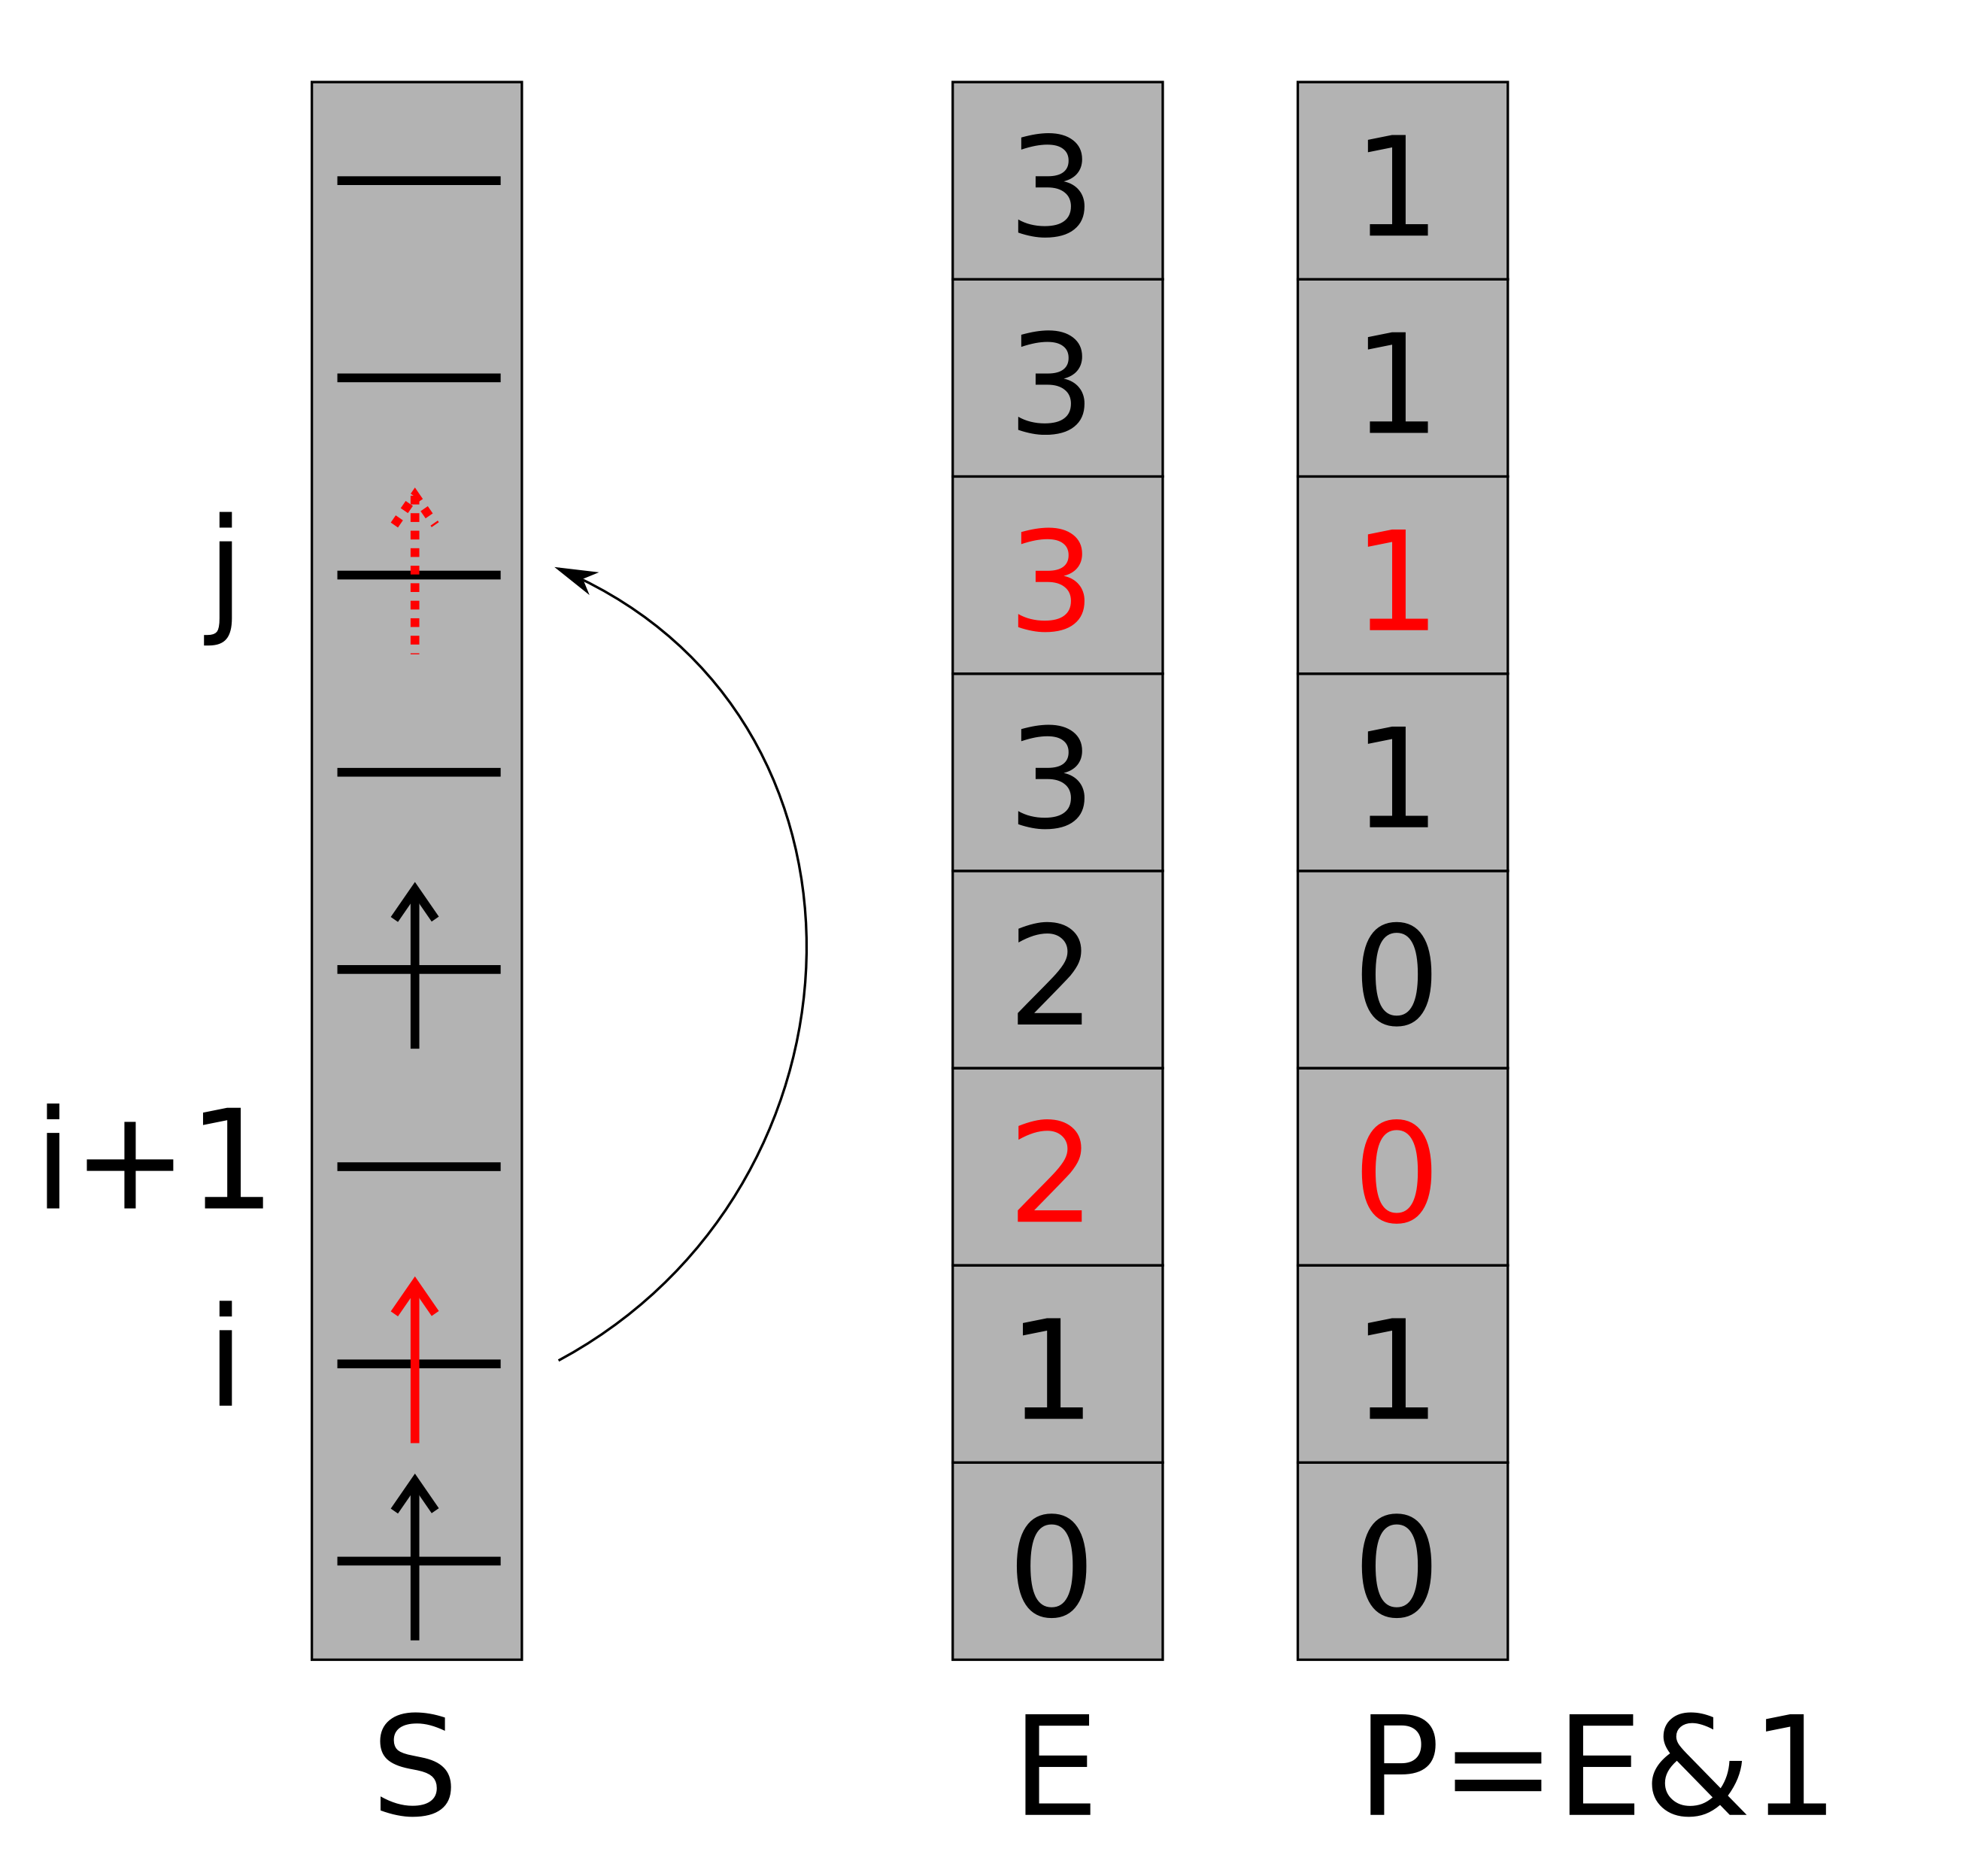
\includegraphics[width=0.65\columnwidth]{figures/determinant_driven/phase}
		\caption[phase mask illustration]{
		Illustrative exemple of phase mask use. $h$ and $p$ are the hole and particle involved in the excitation. $E_i^S$ is the number of electrons in spinorbitals $i$ and below (of same spin), $P_i^S$ is its parity. Because $h>p$, $E_{h-1}^S - E_{p}^S$ gives the number of electrons that are ``crossed'' during the excitation. The phase factor is computed according to Eq.\ref{eq:PHASE_FACTOR}
		}
		\label{generators_selectors}
	\end{center}
\end{figure}


Currently, the \QP does not store a phase mask for each determinant of the wave function, but recomputes it whenever needed before a loop.
The algorithm for computing $P^I$ as a bitstring is shown as algorithm \ref{alg:PHASEMASK}. It uses a trick to get the phase mask of a single integer with logarithmic complexity (loop at line 6 of the algorithm). With $P^0$ a single-integer bitstring for which we want to compute the phase mask, bits being indexed from $0$:

\begin{enumerate}
\item
$P^1 \gets P^0 \oplus \ishft{P^0}{2^0})$.\\
\begin{align}
P^1_i& =
  \begin{cases}
  	p(P^0_i)  & \text{if } i<1 \\
  	p(P_{i-1}^0 + P_{i}^0)   & \text{if } i \geq 1 \\
  \end{cases}
\end{align}
\begin{equation}
P^1_i = p \left (\sum_{j=max(i-1,0)}^{i} P_j^0 \right )
\end{equation}
\item
$P^2 \gets P^1 \oplus \ishft{P^1}{2^1})$.\\
\begin{align}
P^2_i& =
  \begin{cases}
  	p(P^1_i)  & \text{if } i<2 \\
  	p(P_i^1 + P_{i-2}^1)    & \text{if } i \geq 2 \\
  \end{cases}
\end{align}
\begin{equation}
P^2_i = p \left (\sum_{j=max(i-3,0)}^{i} P_j^0 \right )
\end{equation}
\item
$P^3 \gets P^2 \oplus \ishft{P^2}{2^2})$.\\
\begin{align}
P^3_i& =
  \begin{cases}
  	p(P^2_i)  & \text{if } i<4 \\
  	p(P_i^2 + P_{i-4}^2)    & \text{if } i \geq 4 \\
  \end{cases}
\end{align}
\begin{equation}
P^3_i = p \left (\sum_{j=max(i-7,0)}^{i} P_j^0 \right )
\end{equation}
\item
etc...
\end{enumerate}
For a 64-bit integer we have to go to 
\begin{equation}
P^6_{i<64} = p \left (\sum_{j=0}^{i} P_j^0 \right )
\end{equation}
which is the definiton of a phase mask (here indexed from $0$).

%The phase mask as described is
%\begin{equation}
%P = \ISHFT{P^6}{1} \; ;\; P_i = p \left (\sum_{j=0}^{i-1} P_j^0 \right )
%\end{equation}
%but for convenience, the $\text{\texttt{ISHFT}}$ may be omitted. Because in a feasible excitation $\hat T_i^j$ it is known exactly one of $i$ and $j$ is occupied, using $P^6$ directly as the phase mask will result in the computed phases to be systematically flipped, which is transparent. Alternatively, the return value of algorithm \ref{alg:PHASE_FROM_PHASEMASK} can be flipped if used with an ``unshifted'' phase mask.



The method to compute the phase factor associated with a single excitation from a phase mask is shown as algorithm \ref{alg:PHASE_FROM_PHASEMASK}.
With this method, the cost of computing a phase factor ---~after paying the overhead of computing $P$~--- is accessing two bits and applying the \lstinline{IEOR} function to them, in addition to the tests. Unlike the general method, its cost doesn't depend on $\Nint$, and doesn't require to deal with the cumbersome boundaries of 64-bit integers.\phantom{\ref{alg:EXC_DEGREE}}


\subsection{Double excitations}


A double excitation can be expressed as a product of two single excitations.
In the case of an $\uparrow \downarrow$ double excitation, the two single excitations are independent, so the phase factor is merely the product of the phase factors computed for each spin part. 
\begin{equation}
\phase{\ket{I}}{\ordering \excorb{p \bar q}{r \bar s} \ket{I}} = 
\phase{\ket{I}}{\ordering \excorb{p}{r} \ket{I}} \times
\phase{\ket{I}}{\ordering \excorb{\bar q}{\bar s} \ket{I}} 
\end{equation}


There is a slight complication for $\uparrow \uparrow$ or $\downarrow \downarrow$ excitations. The ordering we defined for excitation operators is of importance. In order to write a double excitation as a product of two single excitations, it must be ensured that the ordering matches the one we defined : lowest particle with lowest hole, highest particle with highest hole.

As far as phase computation goes, it is irrelevant which index of an excitation operator is a creation and which is an annihilation. So, for convenience, we can define
\begin{equation}
\tilde T_{ab} = \hat T_a^b + \hat T_b^a
\end{equation}
since at most one of $\hat T_a^b$ or $\hat T_b^a$ is non-zero on a determinant.


Considering a double excitation $\tilde T^2$ involving 4 spinorbitals $p,q,r,s$ of same spin, there are two possible situations, shown in figure \ref{fig:biphasefactor}. 

\begin{itemize}
\item
It can be expressed as two single excitations that do not cross, i.e.
\begin{equation}
\tilde T^2=\tilde T_{pr} \tilde T_{qs} \; ; \; p<r<q<s
\end{equation}
In this case, the numbers of particles in the ranges $]p, r[$ and $]q, s[$ remain unchanged, so we can write
\begin{equation}
\phase{\ket{I}}{\ordering \tilde T^2 \ket{I}} =
\phase{\ket{I}}{\ordering \tilde T_{pr} \ket I} \times
\phase{\ket{I}}{\ordering \tilde T_{qs} \ket I}
\end{equation}

\item
It can be expressed as two single excitations that cross, i.e.
\begin{equation}
\tilde T^2=\tilde T_{pr} \tilde T_{qs} \; ; \; p<q<r<s
\end{equation}
As we can see in figure \ref{fig:biphasefactor}, applying  $\tilde T_{qs}$ results in a particle being created or annihilated in the range $]p,r[$, resulting in a change of parity for the number of particles in that range. Therefore,
\begin{equation}
\phase{\ordering \tilde T_{qs} \ket{I}}{\ordering \tilde T_{pr} \tilde T_{qs} \ket{I}} = -\phase{\ket{I}}{\ordering \tilde T_{pr} \ket{I}}
\end{equation}
\begin{equation}
\phase{\ket{I}}{\ordering \tilde T^2 \ket{I}} = -\phase{\ket{I}}{\ordering \tilde T_{pr} \ket{I}} \times \phase{\ket{I}}{\ordering \tilde T_{ qs} \ket{I}} 
\end{equation}

\end{itemize}



\begin{figure}[h!]
	\begin{center}
		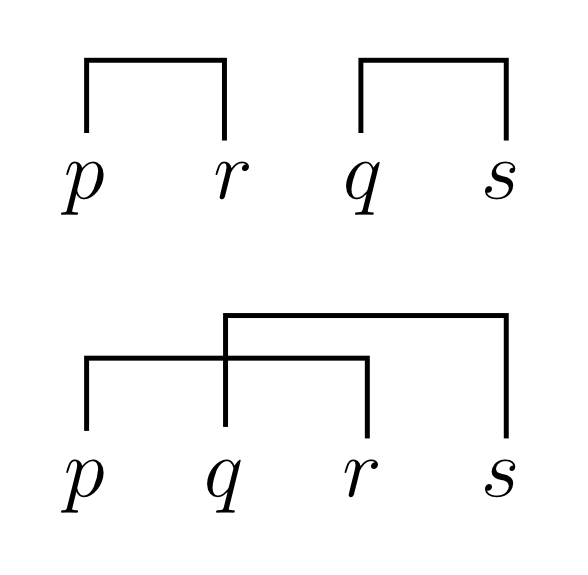
\includegraphics[width=0.2\columnwidth]{figures/determinant_driven/biphasefactor}
		\caption{
		\label{fig:biphasefactor}%
		Crossing of two single excitations.
		The third situation doesn't fit the ordering we imposed on excitation operators. $p \leftrightarrow s$ is either lowest electron to highest orbital, or highest electron to lowest orbital.
		}
	\end{center}
\end{figure}



In practice, because $\text{LIST\_FROM\_BITSTRING}$ returns indices with increasing order, if we determine an excitation operator $\hat T_{pq}^{rs}$ so that $\hat T_{pq}^{rs} \ket I = \pm \ket J$, we know $p<q$ and $r<s$. So for a $\uparrow \uparrow$ or $\downarrow \downarrow$ double excitation, we compute the phase factor from $P^I$ the phase mask associated with $I$, as

%\begin{equation}
% F_{pqrs} = \qty( \max(p,r) > \min(q,s) ) \wedge \qty( \max(q,s) > \min(p,r) )
%\end{equation}


\begin{align}
\phase{\ket I}{\ordering  \hat T_{pq}^{rs} \ket I} = 
\begin{cases}
\kappa & \text{if } \neg \qty( \max(p,r) > \min(q,s) ) \\
-\kappa & \text{if } \qty( \max(p,r) > \min(q,s) )
\end{cases}
\end{align}
with 
%\begin{equation}
%\kappa = \phase{\ket{I}}{\ordering \hat T^r_p \ket I} \phase{\ket{I}}{\ordering \hat T_q^s \ket I}
%\end{equation}

\begin{equation}
\kappa = \text{PHASE\_PHASEMASK}(P^I, p,r) \times \text{PHASE\_PHASEMASK}(P^I, q,s)
\end{equation}
\section{Summary}



Taking advantage of low-level hardware instructions, we are able, for a minimal cost, to find $\hat T$ so that $\hat T \ket I = \ket J$, which yields the $i,j,k,l$ indices of the associated two-electron integral(s). Then, fetching its value can be done quickly using the proposed hash table.
Because of the data structure we are using to store determinants, we also need to compute a phase factor, which can be done efficiently using the introduced phase masks. 

Thanks to the algorithms presented in this chapter, we are able to efficiently compute the matrix elements of $\hat H$, which are the basic ingredients of determinant-driven methods. The instructions and functions we have defined here will be used in the following chapters for many different purposes.

\end{document}
